\documentclass[11pt,a4paper]{article}

\usepackage[T1]{fontenc}
\usepackage[utf8]{inputenc}
\usepackage[polish]{babel}
\usepackage{lmodern}
\usepackage[a4paper,margin=2.5cm]{geometry}
\usepackage{graphicx}
\usepackage{booktabs}
\usepackage{amsmath}
\usepackage{xcolor}
\usepackage{listings}
\usepackage{caption}
\usepackage{float}
\usepackage{tikz}
\usetikzlibrary{arrows.meta,positioning,fit,backgrounds,calc}
\usepackage[colorlinks=true,linkcolor=navy,citecolor=navy,urlcolor=navy]{hyperref}

\definecolor{navy}{RGB}{20,40,120}
\definecolor{codebg}{RGB}{248,248,246}
\definecolor{codekw}{RGB}{40,70,140}
\definecolor{codecom}{RGB}{110,120,110}
\definecolor{codestr}{RGB}{140,80,40}
\definecolor{codenum}{RGB}{140,140,140}

\lstdefinestyle{proj}{
  basicstyle=\ttfamily\scriptsize,
  numbers=left, numberstyle=\tiny\color{codenum}, numbersep=6pt,
  backgroundcolor=\color{codebg},
  keywordstyle=\color{codekw}\bfseries,
  commentstyle=\color{codecom}\itshape,
  stringstyle=\color{codestr},
  frame=single, rulecolor=\color{codenum!50},
  breaklines=true, breakatwhitespace=false, columns=fullflexible,
  keepspaces=true, showstringspaces=false, tabsize=2,
  xleftmargin=1.6em, framexleftmargin=1.2em,
  inputencoding=utf8, extendedchars=true,
  literate={ą}{{\k a}}1 {ę}{{\k e}}1 {ó}{{\'o}}1 {ć}{{\'c}}1 {ł}{{\l}}1 {ń}{{\'n}}1
           {ś}{{\'s}}1 {ź}{{\'z}}1 {ż}{{\.z}}1 {Ą}{{\k A}}1 {Ę}{{\k E}}1 {Ó}{{\'O}}1
           {Ć}{{\'C}}1 {Ł}{{\L}}1 {Ń}{{\'N}}1 {Ś}{{\'S}}1 {Ź}{{\'Z}}1 {Ż}{{\.Z}}1
           {–}{{--}}1 {—}{{---}}1 {„}{{,,}}1 {”}{{''}}1,
}
\lstdefinestyle{pyc}{style=proj, language=Python}
\lstdefinestyle{shc}{style=proj, language=bash}
\lstdefinestyle{plain}{style=proj, numbers=none, xleftmargin=0.5em, framexleftmargin=0.3em}
\lstset{style=proj}

\captionsetup{font=small, labelfont=bf, skip=6pt}
\captionsetup[table]{position=above}
\captionsetup[figure]{position=below}
\setlength{\emergencystretch}{2em}
\renewcommand{\arraystretch}{1.08}

\newcommand{\kod}[1]{\texttt{#1}}
\newcommand{\tabBlunder}{%
\begin{tabular}{llrrr}
\toprule
Tempo & Elo & Z czasem & Pod flagą & Wzrost \\
\midrule
ultrabullet & $<$1200 & 24,8\% & 44,4\% & +79\% \\
ultrabullet & 1200 & 25,3\% & 38,4\% & +52\% \\
ultrabullet & 1600 & 22,1\% & 34,4\% & +56\% \\
ultrabullet & 2000 & 20,2\% & 31,7\% & +57\% \\
ultrabullet & 2400+ & 16,7\% & 29,1\%* & +75\% \\
\addlinespace[2pt]
bullet & $<$1200 & 22,6\% & 32,8\% & +45\% \\
bullet & 1200 & 19,7\% & 29,7\% & +51\% \\
bullet & 1600 & 18,2\% & 27,7\% & +52\% \\
bullet & 2000 & 16,2\% & 26,6\% & +64\% \\
bullet & 2400+ & 13,4\% & 26,7\% & +99\% \\
\addlinespace[2pt]
blitz & $<$1200 & 23,2\% & 33,8\% & +45\% \\
blitz & 1200 & 18,7\% & 29,4\% & +57\% \\
blitz & 1600 & 16,1\% & 26,8\% & +67\% \\
blitz & 2000 & 12,9\% & 24,0\% & +86\% \\
blitz & 2400+ & 10,1\% & 22,4\% & +121\% \\
\addlinespace[2pt]
rapid & $<$1200 & 25,5\% & 38,1\% & +49\% \\
rapid & 1200 & 19,3\% & 31,7\% & +64\% \\
rapid & 1600 & 15,8\% & 27,3\% & +73\% \\
rapid & 2000 & 12,3\% & 24,8\% & +102\% \\
rapid & 2400+ & 8,4\% & 20,7\%* & +147\% \\
\addlinespace[2pt]
classical & $<$1200 & 27,8\% & 0,0\%* & -100\% \\
classical & 1200 & 20,7\% & 17,3\%* & -16\% \\
classical & 1600 & 14,6\% & 22,7\%* & +55\% \\
classical & 2000 & 9,8\% & 22,0\%* & +125\% \\
\addlinespace[2pt]
\bottomrule
\end{tabular}}

\newcommand{\tabComeback}{%
\begin{tabular}{lrr}
\toprule
Tempo & Udział & $n$ \\
\midrule
ultrabullet & 77,2\%* & 1850 \\
bullet & 55,7\% & 49770 \\
blitz & 47,2\% & 104385 \\
rapid & 45,9\% & 73355 \\
classical & 40,4\% & 4394 \\
\bottomrule
\end{tabular}}

\newcommand{\tabThink}{%
\begin{tabular}{llrrr}
\toprule
Tempo & Elo & 0--2 s & 2--10 s & 10+ s \\
\midrule
blitz & $<$1200 & 65,6 & 91,4 & 123,4 \\
blitz & 1200 & 55,7 & 75,8 & 103,5 \\
blitz & 1600 & 50,6 & 67,3 & 92,6 \\
blitz & 2000 & 44,5 & 55,5 & 77,8 \\
blitz & 2400+ & 40,5 & 45,8 & 63,9 \\
\addlinespace[2pt]
bullet & $<$1200 & 80,0 & 103,6 & 126,1 \\
bullet & 1200 & 68,2 & 93,0 & 117,9 \\
bullet & 1600 & 64,0 & 88,9 & 111,9 \\
bullet & 2000 & 60,7 & 83,5 & 98,1 \\
bullet & 2400+ & 57,2 & 75,6 & 109,0* \\
\addlinespace[2pt]
\bottomrule
\end{tabular}}


\title{Analiza partii szachowych z bazy Lichess\\
       w Hadoop Streaming, HDFS i MongoDB\\[0.4em]
       \large Projekt 1 z przedmiotu Big Data}
\author{Jakub Balicki}
\date{2026-11}

\begin{document}
\maketitle
\vspace{-1em}

\section{Cel i dane}
Projekt sprawdza, jak czas na zegarze, tempo gry i poziom Elo wiążą się z jakością ruchów w partiach szachowych. Dane to Lichess Open Database (licencja CC0), wrzesień 2026: początek miesiąca, 5\,500\,001\,981 B po rozpakowaniu (niewielki początkowy wycinek pełnego miesiąca). Część partii ma zapisaną ocenę silnika (\kod{[\%eval]}, w centypionach) i stan zegara (\kod{[\%clk]}), więc jakość ruchu liczymy z tych adnotacji, bez własnego silnika. Wnioski dotyczą więc wyłącznie partii z oceną z tego wycinka. Partie z błędnym wynikiem, bez Elo lub z niepoprawnym \kod{TimeControl} są odrzucane. Tempo wynika z szacowanego czasu partii (baza + 40 $\cdot$ inkrement): ultrabullet $<30$ s, bullet $<180$ s, blitz $<480$ s, rapid $<1500$ s, classical powyżej. Elo dzielimy na pięć kubełków: $<1200$, 1200, 1600, 2000, 2400+.

Trzy pytania, każde to osobny job MapReduce:
\begin{enumerate}
\item \kod{blunder\_in\_trouble}: czy odsetek błędów rośnie, gdy na zegarze zostaje 10 s lub mniej?
\item \kod{comeback\_by\_tc}: jaki udział rozstrzygniętych partii wygrał gracz, który kiedyś miał ocenę gorszą o co najmniej dwa piony?
\item \kod{think\_vs\_cpl}: czy ruchy po dłuższym namyśle mają mniejszą średnią stratę?
\end{enumerate}

\section{Architektura i pipeline}
Archiwum jest pobierane strumieniowo, rozpakowywane w locie i ucinane na granicy partii, a następnie wgrywane do HDFS (z kontrolą SHA-256, żeby nie powtarzać importu). Trzy joby Hadoop Streaming (mappery i wspólny reducer w Pythonie) czytają surowy PGN i zapisują wyniki w HDFS. Agregaty trafiają do MongoDB Atlas, wykresy powstają z plików wynikowych, a lokalna instancja MongoDB (TLS, SCRAM) przechowuje ranking FIDE ze scrapingu oraz metadane importów. Całość działa w Dockerze (Hadoop 3.4.3, MongoDB 7.0.45).

\begin{figure}[H]
\centering
\begingroup\hyphenpenalty=10000\exhyphenpenalty=10000
\resizebox{0.98\textwidth}{!}{%
\begin{tikzpicture}[
  font=\sffamily\scriptsize,
  box/.style={draw, rounded corners=2pt, fill=blue!6, minimum width=2.9cm, minimum height=1.2cm, align=center, text width=2.8cm},
  hbox/.style={box, fill=orange!14},
  dbox/.style={box, fill=green!12},
  fbox/.style={box, fill=gray!14},
  arr/.style={-{Stealth[length=2mm]}, thick},
  lab/.style={font=\sffamily\tiny, above, inner sep=1.5pt}
]
\node[box]  (zst)  at (0,0)     {archiwum Lichess\\\texttt{.pgn.zst}};
\node[box]  (dl)   at (3.7,0)   {\texttt{download.py}\\\texttt{.zst}\,$\to$\,\texttt{.pgn}\\(5,5 GB)};
\node[hbox] (raw)  at (7.4,0)   {HDFS\\\texttt{/user/chess/raw/}\\\texttt{lichess\_2026-09}\\\texttt{.pgn}};
\node[hbox] (mr)   at (11.1,0)  {Hadoop Streaming\\mapper $\to$ shuffle $\to$ reducer};
\node[hbox] (out)  at (14.8,0)  {HDFS\\\texttt{/user/chess/out/}\\wyniki \texttt{part-00000}};
\draw[arr] (zst) -- (dl);
\draw[arr] (dl) -- (raw) node[lab, pos=0.5]{\texttt{put}};
\draw[arr] (raw) -- (mr);
\draw[arr] (mr) -- (out);
\node[dbox] (atlas) at (7.4,-3.2)   {MongoDB Atlas (M0)\\\texttt{mongodb+srv://}\\\texttt{aggregates}};
\node[box]  (load)  at (11.1,-3.2)  {\texttt{load\_aggregates.py}\\upsert \texttt{(analysis, key)}};
\node[box]  (chart) at (14.8,-3.2)  {\texttt{charts.py}\\(matplotlib)};
\node[dbox] (local) at (11.1,-6.4)  {MongoDB lokalna (Docker)\\TLS + SCRAM\\\texttt{fide\_top}, \texttt{import\_runs}};
\node[fbox] (plots) at (14.8,-6.4)  {wykresy\\\texttt{plots/*.png}};
\draw[arr] (out.south) -- (chart.north) node[lab, pos=0.5, right, above=0pt]{\texttt{hdfs get}};
\draw[arr] (out.south west) -- ++(0,-0.9) -| (load.north);
\draw[arr] (load) -- (atlas) node[lab, pos=0.5]{agregaty};
\draw[arr] (load) -- (local) node[lab, pos=0.5, right, above=0pt]{metadane};
\draw[arr] (chart) -- (plots);
\node[fbox] (fide)  at (0,-6.4)   {\texttt{ratings.fide.com}\\listy rankingowe (HTML)};
\node[box]  (scr)   at (3.7,-6.4) {\texttt{scrape\_fide.py}\\requests + BeautifulSoup};
\draw[arr] (fide) -- (scr);
\draw[arr] (scr) -- (local) node[lab, pos=0.5]{upsert, TLS};
\begin{pgfonlayer}{background}
  \node[draw, dashed, rounded corners=3pt, inner sep=7pt, fit=(fide)(scr),
        label={[font=\sffamily\tiny, anchor=south west]north west:gałąź niezależna: scraping}] {};
\end{pgfonlayer}
\end{tikzpicture}}
\endgroup
\caption{Przepływ danych. Pomarańczowe bloki działają w kontenerze Hadoop, zielone to bazy MongoDB. Agregaty trafiają do Atlasu, a do lokalnej bazy trafiają ranking FIDE i metadane importów.}\label{fig:flow}
\end{figure}


\paragraph{Joby MapReduce.} Mapper czyta partie, wywołuje funkcję analizy i wypisuje linie „klucz, tabulator, liczby”; reducer sumuje liczniki po kluczu, a odsetki i średnie liczone są dopiero po jobie. Plik ma jeden split wejścia, żeby partia PGN nie została przecięta w połowie. Zapis do Atlasu to upsert po unikalnym indeksie \kod{(analysis, key)}, więc powtórny import nie dubluje dokumentów. Wyniki to 126 wierszy: 49 (błędy), 5 (powroty), 72 (czas namysłu).

\paragraph{Definicje miar.}
\emph{Strata} ruchu to $\max(0,\ c_\text{przed}-c_\text{po})$ z perspektywy grającego. \emph{Błąd} to strata co najmniej 100 cp; ruch jest \emph{pod flagą}, gdy zegar po ruchu wynosi najwyżej 10 s. Ruchy bez pary ocen liczbowych (w tym z matem) lub bez zegara są pomijane. \emph{Powrót}: zwycięzca partii rozstrzygniętej miał kiedykolwiek ocenę $\le -200$ cp (biały) lub $\ge +200$ cp (czarny); mianownikiem są wszystkie rozstrzygnięte partie z oceną, więc to nie jest prawdopodobieństwo wygranej z gorszej pozycji. \emph{Czas namysłu} to różnica własnych zegarów powiększona o inkrement, w koszykach 0--2 s, 2--10 s, 10+ s.

\section{Wyniki}
Komórki z mniej niż 1000 ruchów oznaczono gwiazdką (tabele) lub kreskowaniem (rysunki) i nie wyciągamy z nich wniosków.

\subsection{Błędy pod flagą}
\begin{table}[H]
\centering
\caption{Odsetek błędów (strata $\ge100$ cp) z czasem i pod flagą (zegar $\le10$ s); wzrost to zmiana względna. Gwiazdka: któraś grupa ma poniżej 1000 ruchów.}\label{tab:blunder}
\small
\tabBlunder
\end{table}

Przykład: w blitzu przy Elo 1200--1599 błędów jest 18,7\% z czasem i 29,4\% pod flagą (+57\%); w bulleciu 19,7\% wobec 29,7\% (+51\%). Rysunek~\ref{fig:blunder} pokazuje te same dane graficznie.

\begin{figure}[H]
\centering
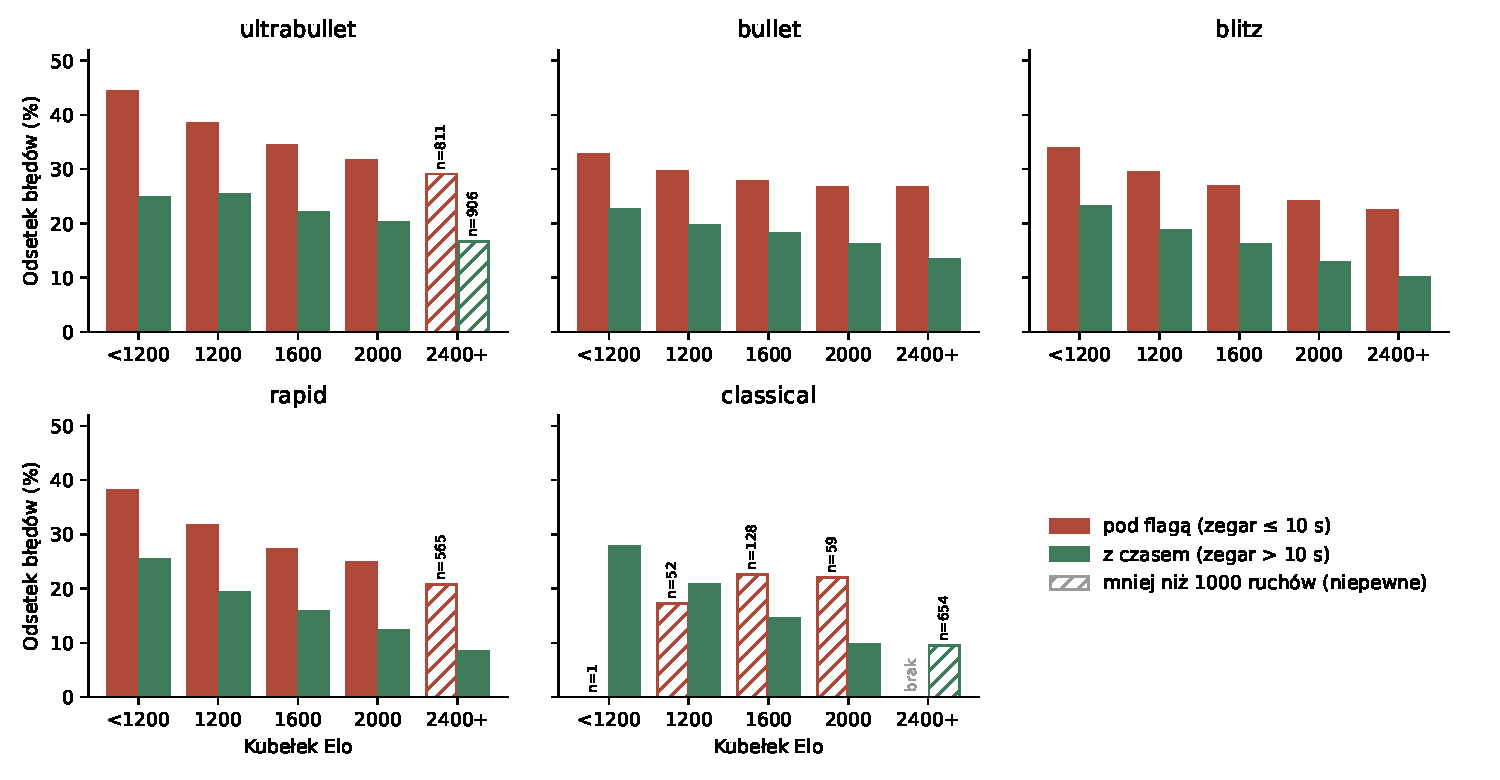
\includegraphics[width=0.9\textwidth]{figures/blunder.pdf}
\caption{Odsetek błędów pod flagą i z czasem według tempa i Elo. Kreskowane słupki: poniżej 1000 ruchów.}\label{fig:blunder}
\end{figure}

\subsection{Powroty}
\begin{table}[H]
\centering
\caption{Udział rozstrzygniętych partii z oceną, w których zwycięzca był kiedyś gorszy o co najmniej dwa piony.}\label{tab:comeback}
\tabComeback
\end{table}

\begin{figure}[H]
\centering
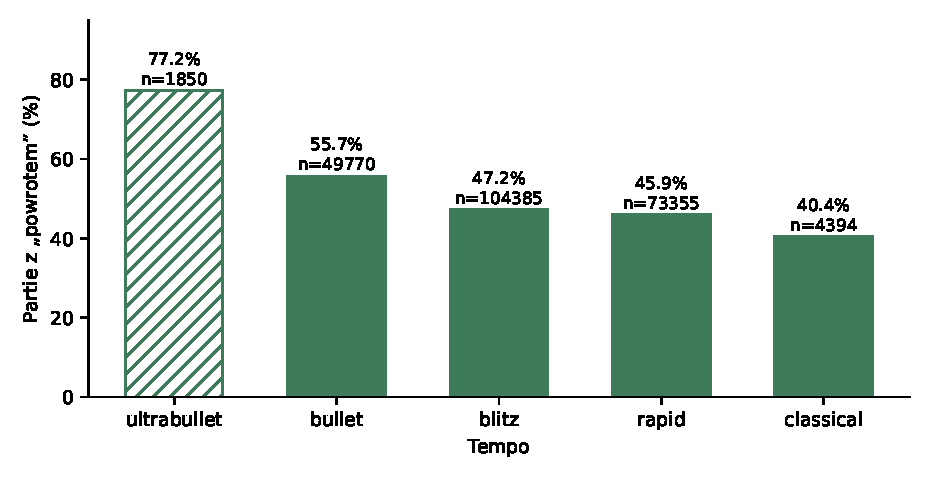
\includegraphics[width=0.65\textwidth]{figures/comeback.pdf}
\caption{Udział partii z powrotem według tempa. Kreskowany słupek (ultrabullet) ma bardzo małą próbę.}\label{fig:comeback}
\end{figure}

\subsection{Czas namysłu}
Tabela~\ref{tab:think} podaje średnią stratę w koszykach czasu dla blitza i bulleta (wycinek wyników), a rys.~\ref{fig:think} wszystkie tempa.

\begin{table}[H]
\centering
\caption{Średnia strata centypionów na ruch w koszykach czasu namysłu, blitz i bullet.}\label{tab:think}
\small
\tabThink
\end{table}

\begin{figure}[H]
\centering
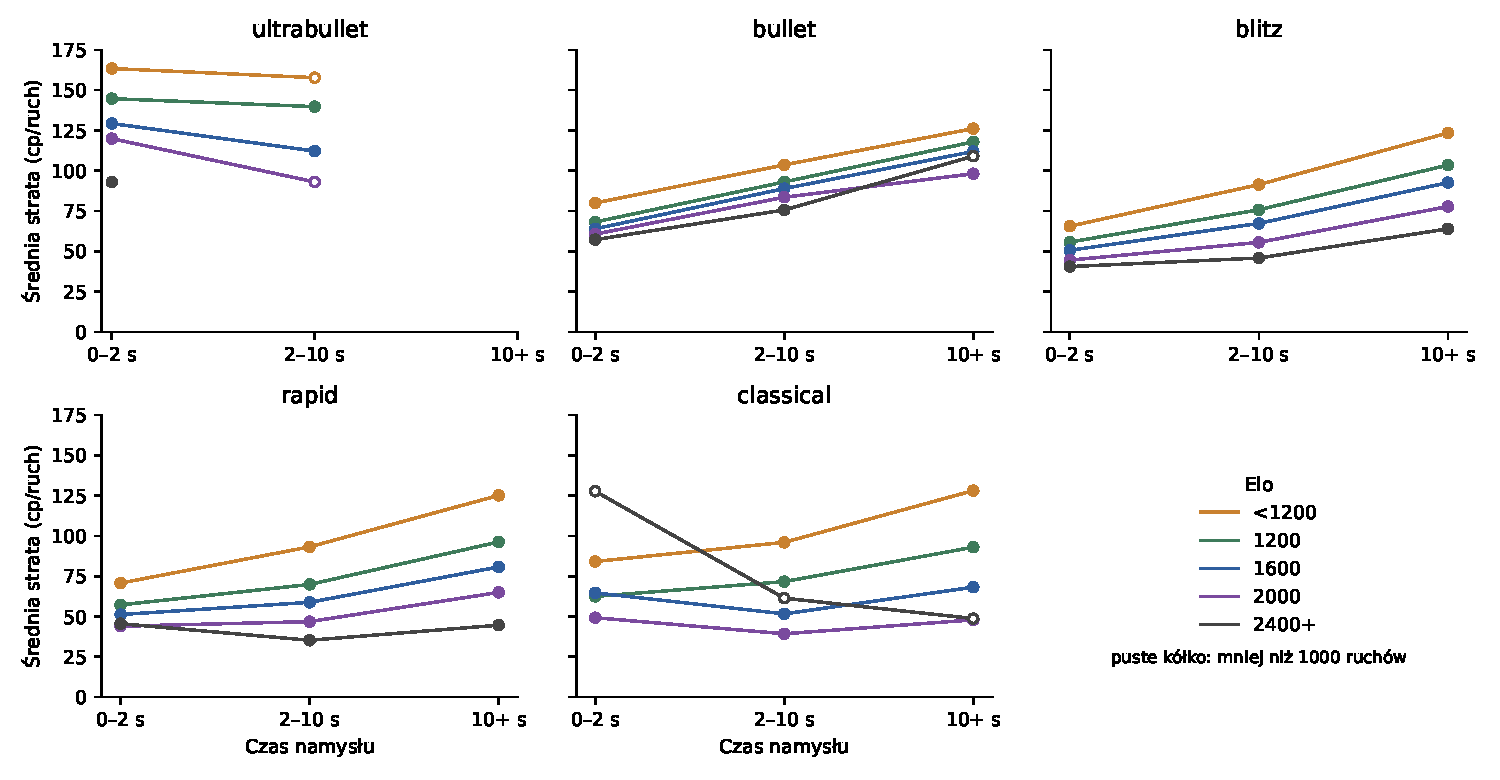
\includegraphics[width=\textwidth]{figures/namysl.pdf}
\caption{Średnia strata centypionów w zależności od czasu namysłu, osobno dla tempa i Elo. Puste kółka: poniżej 1000 ruchów.}\label{fig:think}
\end{figure}


\section{Wnioski}
\begin{itemize}
\item Pod flagą ruchy są częściej błędami niż z czasem we wszystkich komórkach o dużej próbie. W blitzu względny wzrost rośnie z Elo, od +45\% ($<1200$) do +121\% (2400+), ale to w części efekt niskiej podstawy najsilniejszych graczy (10,1\% z czasem w blitzu 2400+).
\item Udział partii z powrotem maleje od bulleta (55,7\%) przez blitz (47,2\%) i rapid (45,9\%) do klasycznych (40,4\%). Wynik ultrabulleta (77,2\%) opiera się na próbie 1850 partii.
\item W blitzu i bulleciu średnia strata rośnie z czasem namysłu we wszystkich kubełkach Elo, co raczej odzwierciedla trudność pozycji (dłużej myśli się w trudnych) niż szkodliwość myślenia. W rapidzie i partiach klasycznych wzór jest nieregularny.
\item Wyniki są opisowe i dotyczą początkowego wycinka miesiąca z partii z oceną silnika; nie wskazują przyczyn.
\end{itemize}

\end{document}
